The CAM module in hardware will be connected to the ZYNQ through a AXI LITE interconnect. The AXI LITE has signals that are not relevant to the logic inside the Content Addressable Memory and because of that the hardware implementation of the CAM should be divided in to a CAM and a CAM logic unit.

The CAM wraps the CAM Logic Unit module. This wrapper module will be connected with the AXI Interconnect through a AXI LITE interface and will filter the received data from this interface to provide the CAM Logic Unit module only the necessary signals. The CAM module with the CAM Logic Unit module instantiation is illustrated in the figure \ref{fig:CAM_HwLogic}.

\begin{figure} [H]
	\centering
	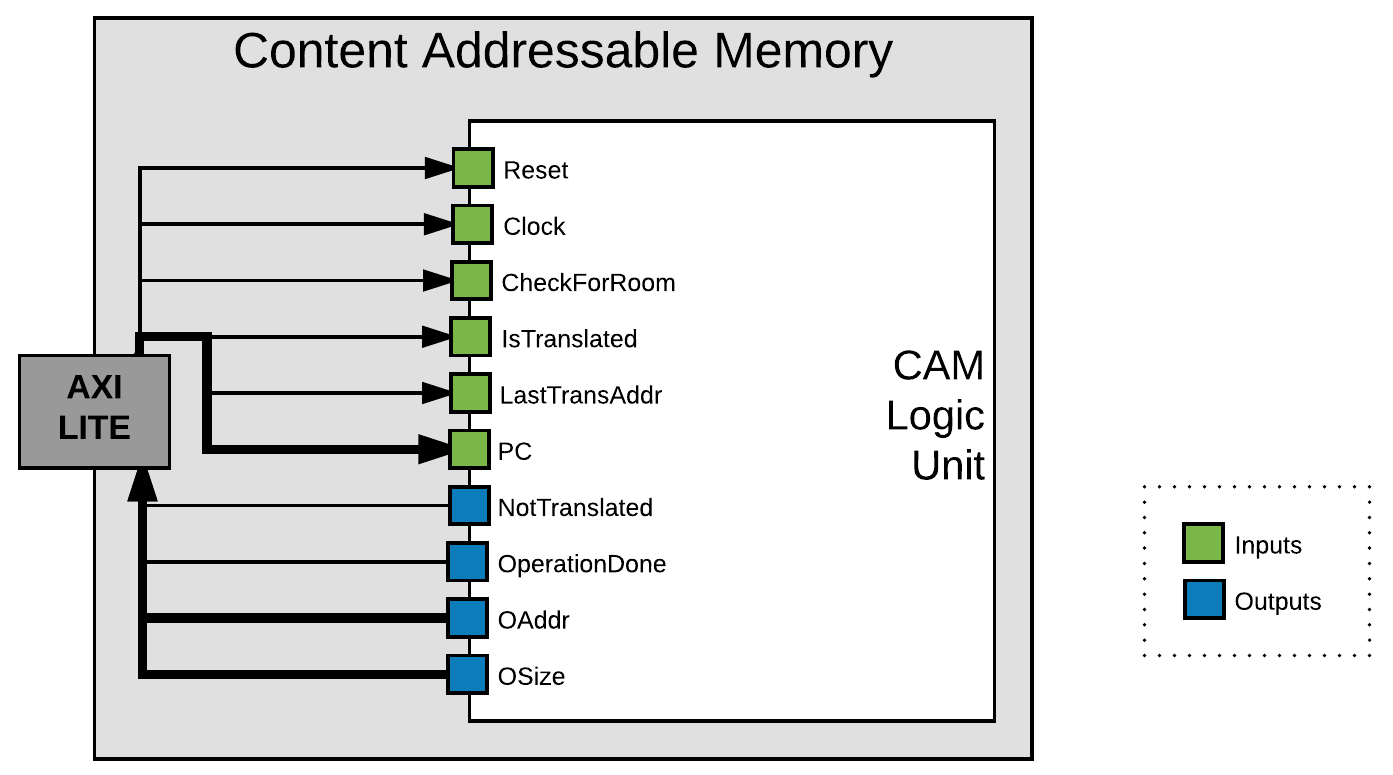
\includegraphics[scale = 0.25]{Images/CAM_HwLogic.png}
	\caption{CAM Logic Unit}
	\label{fig:CAM_HwLogic}
\end{figure}

